\begin{abstract}
Sprint-risk models are usually trained on a present-day Jira export, which shows how a sprint ended rather than what the team knew when it began, and each study reports its own features on its own data. We state formally what a feature may use at prediction time and when an outcome can be measured, and work out four simple consequences that we check against the data. The measurability rule removes three TAWOS projects whose issues are mostly closed without a resolution date. On the remaining \NSprints{} sprints from \NProj{} projects, scored under one time-ordered protocol for five outcomes, progress counts carry the in-sprint signal. Burndown-shape features rank sprints worse by 0.13 to 0.19 AUC and add nothing when combined with progress counts, across projects and within them. Team history beats committed scope for serious spillover by \dPTHistSs{} AUC, but nearly all of that gain comes from telling teams apart. Within a project it falls to \dPWHistSs{}, with an interval that includes zero, as a binomial model with one completion rate per team implies. That model learns nothing and ranks sprints about as well as gradient boosting, but its probabilities are too extreme. Four new planning-time features add \dPTNewSp{} AUC for spillover, within projects too, but the gain does not hold on the \ConfProj{} projects that did not shape our hypotheses. Nothing we tried predicts late closure well, and on ten outside projects we see no sign that the history gains carry over.
\end{abstract}

\begin{IEEEkeywords}
Agile software development, data leakage, data quality, Jira, machine learning, mining software repositories, Scrum, sprint risk
\end{IEEEkeywords}

\section{Introduction}

\IEEEPARstart{A}{} Scrum team commits to a set of issues at the start of each sprint. Some sprints end with work left over, and some are closed in Jira days after their planned end. Both are visible to everyone once the sprint is over. The useful question is whether they can be seen coming, at planning or early in the sprint, from what the tracker already records.

Several studies have tried \cite{choet2018,sprint2vec,hearty2009,perez2024,obike2025}, and industrial work has studied what makes delivery late \cite{kula2022}. Their results are hard to use for three reasons. The first is hindsight. A Jira export is a snapshot taken years later: an issue's sprint field, story points and status are the final values unless the change log is replayed. A model trained on the snapshot can learn from facts that did not exist at planning \cite{kaufman2012,kapoor2023}. The second is measurement. A label such as ``work left over'' depends on when each issue was finished, and a tracker does not always record that. The third is comparability. Every study brings its own features, labels, data and protocol, so if one paper reports a good AUC with burndown features and another with iteration counts, nobody can tell which kind of signal does the work.

Our earlier work \cite{abusharkh2027} rebuilt the board as it stood on the first day of each sprint for eight TAWOS projects \cite{tawos}. Here we turn that reconstruction into a benchmark. We extend it to every TAWOS project with enough sprints, check that the outcomes can be measured, and score the feature families side by side on the same sprints, labels and split. The contributions are as follows.
\begin{enumerate}
\item \emph{A head-to-head benchmark with fair comparisons} (Sections~\ref{sec:protocol} and \ref{sec:results}). Committed scope, team history, four new planning-time features, in-sprint progress counts, burndown-shape features after P\'erez Castillo et al.\ \cite{perez2024}, and the iteration counts of Choetkiertikul et al.\ \cite{choet2018} that a public export supports, compared both as stand-alone sets and by what each adds to the others.
\item \emph{A measurability check} (Section~\ref{sec:setup}). In three TAWOS projects most sprint issues are closed without a resolution date. Removing them changes which of our hypotheses hold, so any study of spillover on TAWOS needs this check.
\item \emph{Pooled and within-project ranking} (Section~\ref{sec:within}). AUC in this literature, ours included, is pooled over projects, so it also rewards telling teams apart. Scored only within projects, the in-sprint findings hold but most of the planning-time history gain disappears. This matters for any tool that a single team would use on its own sprints.
\item \emph{A formal setting} (Section~\ref{sec:theory}). Admissible features and measurable outcomes are defined on the event log, with four elementary consequences: how empty sprints inflate ROC-AUC, the cost ratio a Youden threshold assumes, a binomial model of which spillover label history can help with, and a beta-binomial extension that says when that model's probabilities can be trusted.
\item \emph{Three candidate labels with a verdict on each, a confirmation set, an outside test and a decision analysis.} Of the three new labels, only serious spillover can be ranked beyond committed scope; seriously late and scope churn cannot, and we report them as negative results. Every hypothesis test is repeated on the projects that played no part in writing the hypotheses, with a multiple-testing correction, and the gains are translated into what a warning is worth.
\end{enumerate}

The short answer is that progress counts carry the in-sprint signal and burndown shape adds nothing. At planning time, team history mostly tells teams apart, not a team's good sprints from its bad ones, and most of what a learned model does is estimate one number per team. We see no sign that the history gains carry to another organisation. Our plan and hypotheses are in the first commit of the repository, made before the full run. We report where they failed and mark every analysis added later.

\section{Related Work}
\label{sec:related}

\subsection{Predicting sprint and iteration outcomes}

Choetkiertikul et al.\ \cite{choet2018} predicted how much of an iteration's committed work would be delivered, using iteration-level counts (issues and points at start, added, removed, done, to do) together with issue-level and team features, on open-source projects. The same group predicted risks and delays at the level of single issues \cite{choet2015,choet2017}, and Sprint2Vec \cite{sprint2vec} learns a sprint embedding from issue text and developer activity. Hearty et al.\ \cite{hearty2009} modelled velocity in XP with a dynamic Bayesian network. In industry, Kula et al.\ studied the factors behind on-time delivery in large-scale agile development \cite{kula2022} and predicted delays of user stories from team dynamics \cite{kula2021}. More recently, P\'erez Castillo et al.\ \cite{perez2024} graded finished sprints from eleven burndown-shape indicators (R1 to R11) computed in their Worki tool, and Obike et al.\ \cite{obike2025} scored sprint deliverability with a weighted index. Effort estimation \cite{choet2019,porru2016,fu2023,tawosi2023} is a neighbouring problem: it predicts the size of an issue, not the fate of a sprint.

All of this work rests on issue-tracker data, and public Jira datasets \cite{tawos,ortu2015,montgomery2022} have made it reproducible. They are, however, exports taken long after the fact. The studies above differ in data, labels and validation, and in how strictly features are limited to what was known at prediction time. In cross-validation over iterations, a training fold can hold iterations that happened after the test ones \cite{choet2018}. No study compares the feature families on common data. We do not claim to reproduce any of them. We implement the parts of two feature families that a public export supports and score them on our sprints, so what we measure is the feature families rather than the papers that proposed them.

\subsection{Leakage and time-aware evaluation}

Leakage, where a model sees information it would not have when deployed, is a known cause of inflated results \cite{kaufman2012,kapoor2023}. In software analytics, the choice of validation technique changes the performance a defect model appears to have \cite{tanti2017}, random splits mix past and future \cite{bangash2020,falessi2020}, and labels that are only known later leak into features \cite{jimenez2019}. Shepperd et al.\ \cite{shepperd2014} found that which research group ran a defect-prediction study explained more of the variation in reported performance than the choice of learner. A common protocol on common data is the remedy we apply here. Our earlier work \cite{abusharkh2027} showed, on eight TAWOS projects, that two reproduced leakage mistakes inflated F1 by up to 0.24 and that shuffling sprints before splitting added 0.07 AUC. The present paper reuses that reconstruction but none of its results.

\subsection{Predictive monitoring and warnings as decisions}

Predictive process monitoring \cite{marquez2018,teinemaa2019} faces the same problem with event logs: it predicts the outcome of a running case from a prefix of its events, and benchmarks compare methods on common logs \cite{difrancesco2018,teinemaa2019}. Our in-sprint checkpoints are prefixes in this sense. Alarm-based monitoring \cite{fahrenkrog2022} treats a warning as a decision with a cost, which is the view we take in Section~\ref{sec:theory}.

\subsection{Ranking, thresholds and calibration}

ROC-AUC measures ranking \cite{fawcett2006}. It says nothing about where to set a threshold, and its use for comparing classifiers has known limits \cite{hand2009,hernandez2012}. A cost-optimal threshold for a calibrated score follows from the costs alone \cite{elkan2001}, which is why calibration matters. The Brier score \cite{brier1950} and the calibration slope \cite{vancalster2019} measure it, and boosted trees are known to produce distorted probabilities unless checked \cite{niculescu2005}.


% Formal setting. Every number here comes from tables/numbers.tex, written by jr/tables.py
% from results/<cohort>/theory_numbers.json, and is checked by jr/theory_checks.py.

\section{Formal Setting}
\label{sec:theory}

This section fixes what ``no hindsight'' means for a Jira export and derives three consequences. Each one turns a pattern that is easy to miss into a prediction the experiments can check: how empty sprints inflate ROC-AUC, why a threshold fitted on one group of teams does not carry to another, and how the two spillover labels should differ.

\subsection{The event log and the sprint state}

A Jira export is an event log $\mathcal{E} = \{(i, f, v^{-}, v^{+}, t)\}$: issue $i$ had field $f$ changed from $v^{-}$ to $v^{+}$ at time $t$. With each issue's creation time $\gamma_i$ and resolution time $r_i$ (undefined while the issue is open), the log gives the value of any field at any time by replaying the changes in order. Write $\mathcal{E}_{\le t}$ for the events up to time $t$, and $\mathcal{F}_t$ for what they tell us together with the sprint calendar, which is fixed at planning. A sprint $s$ has a start $a_s$, a planned end $b_s$ and a closure time $c_s$.

The committed set is the board at the start,
\begin{equation}
C_s = \{\, i : s \in \mathrm{sprint}_i(a_s),\ \gamma_i \le a_s,\ r_i \not< a_s \,\},
\label{eq:committed}
\end{equation}
where $\mathrm{sprint}_i(t)$ is the issue's sprint field at time $t$ as replayed from $\mathcal{E}_{\le t}$. The outcomes are read off the end state. With $n_s = |C_s|$ and the carry ratio
\begin{equation}
\rho_s = \frac{|\{ i \in C_s : r_i > b_s \}|}{n_s},
\end{equation}
spillover is $y^{\mathrm{sp}}_s = \mathbf{1}[\rho_s > 0]$, serious spillover is $y^{\tau}_s = \mathbf{1}[\rho_s \ge \tau]$, late closure is $y^{\mathrm{late}}_s = \mathbf{1}[c_s - b_s > \delta]$ with $\delta$ one day (three for ``seriously late''), and scope churn is $\mathbf{1}[m_s / n_s \ge \theta]$, where $m_s$ counts issues added after $a_s$ and still in the sprint at $b_s$.

\subsection{Admissible features}

\begin{definition}[Admissible feature]
A feature $x(s, t)$ for sprint $s$ at prediction time $t$ is admissible if it is a function of $\mathcal{F}_t$ alone, that is, of $\mathcal{E}_{\le t}$ and the sprint calendar.
\end{definition}

Two common practices break this rule. First, a history feature that summarises an earlier sprint $u$ of the same project is admissible at $a_s$ only if $u$'s outcome was known by then, $\max(b_u, c_u) \le a_s$. A ``previous sprint'' picked by start date alone breaks this whenever sprints overlap, which happens for \OverlapShare\% of the sprints in our cohort. Second, a field read from the static export is $\mathcal{F}_\infty$-measurable, not $\mathcal{F}_{a_s}$-measurable. Wherever the log records no change for a field, the replay has to fall back on a value that may postdate planning. We record the share of committed issues affected, $\phi_s$, and repeat the main comparisons on sprints with $\phi_s = 0$. Issue type, priority and assignee are left out altogether, because the export only holds their final values.

\subsection{Empty sprints inflate ROC-AUC}

A sprint with $n_s = 0$ cannot spill, so it is a negative by construction. Keeping such sprints in a spillover evaluation rewards the model for something it did not have to learn.

\begin{proposition}
\label{prop:auc}
Split the negatives of a test set into structural negatives $N_0$ and ordinary negatives $N_1$, and let $\pi_0 = |N_0| / (|N_0| + |N_1|)$. Then
\begin{equation}
\mathrm{AUC}_{\mathrm{all}} = \pi_0\, A_0 + (1 - \pi_0)\, \mathrm{AUC}_{N_1},
\label{eq:aucmix}
\end{equation}
where $A_0$ is the probability that a random positive outscores a random structural negative, and $\mathrm{AUC}_{N_1}$ is the AUC on the positives and ordinary negatives alone. If the model ranks every structural negative below every positive, $A_0 = 1$ and the inflation is $\pi_0 (1 - \mathrm{AUC}_{N_1})$.
\end{proposition}

\begin{proof}
AUC is the probability that a random positive outscores a random negative. Conditioning on which kind of negative is drawn gives (\ref{eq:aucmix}).
\end{proof}

The decomposition is elementary. Its use is that it puts an exact number on the inflation.

On our time-split test set the full population has \NegAll{} negatives, and \NegStruct{} of them commit nothing, so $\pi_0 = \PiZero$. The model's AUC on nonempty sprints is \AucNonempty. With $A_0 = 1$, (\ref{eq:aucmix}) predicts \AucPred{} for the full population; the observed value is \AucAll, and the measured $A_0$ is \AZero. The gap of \Inflation{} between the two headline numbers is entirely the empty sprints. Any study that keeps them in the denominator reports this gap as skill.

\subsection{Why a fitted threshold does not travel}

Youden's index picks the threshold that maximises sensitivity plus specificity, which is the same as minimising $\mathrm{FNR} + \mathrm{FPR}$. With prevalence $\pi$, a miss cost $c_{\mathrm{FN}}$ and a false-alarm cost $c_{\mathrm{FP}}$, the expected cost per sprint is $\pi c_{\mathrm{FN}} \mathrm{FNR} + (1 - \pi) c_{\mathrm{FP}} \mathrm{FPR}$. This is proportional to $\mathrm{FNR} + \mathrm{FPR}$ exactly when
\begin{equation}
\frac{c_{\mathrm{FN}}}{c_{\mathrm{FP}}} = \frac{1 - \pi}{\pi}.
\label{eq:youden}
\end{equation}

\begin{proposition}
\label{prop:youden}
A Youden threshold fitted on a population with prevalence $\pi_{\mathrm{train}}$ is cost-optimal on a population with prevalence $\pi$ only if the implied cost ratio (\ref{eq:youden}) is the same, that is, only if $\pi = \pi_{\mathrm{train}}$. For a calibrated score the cost-optimal rule warns when $p \ge p^{*} = c_{\mathrm{FP}} / (c_{\mathrm{FP}} + c_{\mathrm{FN}})$, which does not depend on prevalence. A fixed score threshold carried to a team with lower prevalence therefore acts like a rule that prices a miss at only $(1 - \pi_{\mathrm{train}}) / \pi_{\mathrm{train}}$ false alarms, and its sensitivity falls with $\pi$.
\end{proposition}

The link between a threshold rule and the cost ratio it implies is standard in the ROC literature \cite{hernandez2012}. What we add is its use to explain why a threshold that worked on TAWOS misses most failures on some new teams.

For late closure the training prevalence is \TrainPrev, so the implied ratio is \TrainRatio. On the \ExtProjects{} testable outside projects the same threshold meets prevalences from \PrevMin{} to \PrevMax, where (\ref{eq:youden}) would call for ratios from \RatioMin{} down to \RatioMax. The observed sensitivity runs from \SensMin{} to \SensMax, with a rank correlation of \SpearmanPS{} with prevalence. The ranking travels because AUC does not depend on a threshold; the threshold does not travel. A deployment has to recalibrate it per team or set it from stated costs.

\subsection{A minimal model of the two spillover labels}

Suppose each committed issue of sprint $s$ is finished by the planned end independently with probability $q_s$, a property of the team and the period rather than of the issue. The number left unfinished is then $\mathrm{Binomial}(n_s, 1 - q_s)$, and
\begin{align}
\Pr[y^{\mathrm{sp}}_s = 1] &= 1 - q_s^{\,n_s}, \label{eq:any}\\
\mathbb{E}[\rho_s] &= 1 - q_s, \qquad \mathrm{Var}[\rho_s] = \frac{q_s (1 - q_s)}{n_s}. \label{eq:ratio}
\end{align}
Two predictions follow. By (\ref{eq:any}) the ``any'' label is driven by $n_s$ and saturates fast: at the cohort's median carry ratio, \CarryMedian, $q_s \approx \Qhat$ and a sprint of three issues already spills with probability \PSpillThree. The median nonempty sprint commits \MedianIssues{} issues, and \NonemptySpill\% of nonempty sprints spill. So committed scope should carry most of what can be known about plain spillover. By (\ref{eq:ratio}) a threshold label on $\rho_s$ is driven by $1 - q_s$, the team's completion rate, with $n_s$ entering only through the variance. Serious spillover should therefore depend on planning-time history and capacity rather than on scope, and the gap between scope-only and history-aware models should be larger for it than for plain spillover. Section~\ref{sec:results} tests both. The model ignores dependence between issues and scope changes during the sprint. It is a reading aid, not a claim about how teams work.

\subsection{Warnings as decisions}

A warning raised at checkpoint $c$ costs $\kappa$ and, if the sprint would otherwise fail, averts a fraction $e(c)$ of the failure cost $F$, with $e$ falling as $c$ grows. Warning at calibrated risk $p$ has expected cost $\kappa + F p (1 - e(c))$ against $F p$ for staying silent, so the warning pays when
\begin{equation}
p \ge \frac{\kappa}{e(c)\, F}.
\label{eq:warn}
\end{equation}
The bar rises as the sprint goes on, because a late warning saves less. An in-sprint model is useful only where its gain in ranking outpaces the fall in $e(c)$. Because (\ref{eq:warn}) needs a calibrated $p$, we report calibration beside AUC.


\section{Data and Reconstruction}
\label{sec:setup}

\subsection{Cohort}

TAWOS \cite{tawos} holds Jira data from open-source projects; \NProjSprints{} of them have sprints. We count a sprint as usable if it is closed, has start, end and completion dates, and neither the end nor the completion is before the start. \NProjThirty{} projects have at least 30 usable sprints. Three of them (MongoDB Compass and the MongoDB C++ and Java drivers) are also in our outside test set, which we pulled from MongoDB's live Jira, so we drop them from TAWOS. That leaves \NProjExport{} projects.

\subsection{Measurability check}

We checked the rule of Section~\ref{sec:theory} per project after the first full run, when three projects showed most of their sprints finishing nothing, and then reran the cohort. The check measures the share of issues ever placed in a sprint whose status is closed, done, resolved or complete but which have no resolution date. Three projects stand out: Atlassian Jira Cloud (\UnrecA\%), Atlassian Confluence Cloud (\UnrecB\%) and Apache MXNet (\UnrecC\%). In every other project the share is at most \UnrecOtherMax\%, so any cut-off between 1\% and 56\% picks the same three projects. In those three projects most sprints appear to finish nothing (Fig.~\ref{fig:carry}), because closed issues without a date count as never finished. We exclude them. The rule and its cut-off were set before the cohort was rerun, and the cut-off involves no choice, since nothing lies between 1\% and 56\%. Two other projects, Appcelerator Daemon and Hyperledger Indy Node, also show sprints that finish nothing, but their unfinished issues are genuinely open in the export, so the check gives no reason to drop them; we report the main comparisons without them as a robustness check.

\begin{figure}[!htb]
\centering
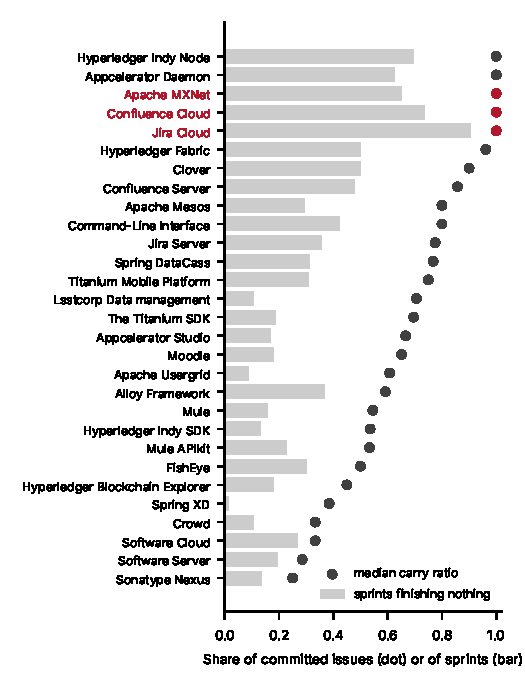
\includegraphics[width=\columnwidth]{fig_carry.pdf}
\caption{Per project, before the measurability check: median share of committed issues left unfinished at the planned end (dot) and share of sprints that finish none of their committed issues (bar). Red: the three projects where most sprint issues are closed without a resolution date.}
\label{fig:carry}
\end{figure}

The cohort is the remaining \NProj{} projects. After dropping each project's first sprint as a cold start, it has \NSprints{} sprints from \DateFrom{} to \DateTo, between \SprintMin{} and \SprintMax{} per project (median \SprintMed). Of these, \NNonempty{} commit at least one issue; we call them nonempty. Before the check, \FullNothingPct\% of nonempty sprints finished none of their committed issues; after it, \CleanNothingPct\%.

The outside set is the ten projects used in our earlier study: MariaDB MaxScale and ColumnStore, and eight MongoDB projects, exported from the organisations' public Jira and converted to the TAWOS layout. All ten pass the measurability check. They are used only for testing.

\subsection{Reconstruction}

For every sprint we replay the Sprint and Story Points fields of every issue back to the sprint's start and form the committed set (\ref{eq:committed}). Issues added later, issues removed later, and their story points at the start all come from the replay. Where an issue has no recorded story-point change, the replay falls back on the exported value; on average \FallbackMean\% of a sprint's committed issues are affected. Two custom fields are excluded from the replay: ``Actual Story Points'' in Spring XD, which is recorded after the work, and a retired duplicate in Moodle.

\emph{Reconstruction check.} No public record shows the board as it stood at each sprint start, so the replay cannot be compared with ground truth. It can be checked for consistency: replaying an issue's log forward must end in the values the export shows. For story points it does in \RecPointsAgree\% of the \RecPointsN{} issues with a story-point history. For the sprint field it does in \RecSprintAgree\% of the \RecSprintBoth{} issues where both the log and the export name a sprint of the cohort. For another \RecExportEmpty{} issues the export shows no sprint although the log's last event names one; the replay follows the log. Of the issues ever placed in a sprint, \RecHistoryPct\% have a sprint history; for the rest the replay has to take the exported sprint as the sprint at the start, the sprint-field counterpart of the story-point fallback. We repeat the main comparisons on projects where at least 85\% of such issues have a history (Section~\ref{sec:robust}).

\section{Outcomes, Features and Protocol}
\label{sec:protocol}

\subsection{Outcomes}

Table~\ref{tab:labels} lists the five outcomes. Late closure and spillover are carried over from our earlier work. The other three are new.

\emph{Serious spillover} asks how much was left over, not whether anything was. We fixed its primary threshold at a carry ratio of 30\% before seeing the full cohort. That was a poor choice: the median nonempty sprint leaves \CarryMedPct\% of its committed issues unfinished, so the label is \PosSs\% positive, not far from plain spillover (\PosSp\%). The median-based version (carry ratio above the training-set median, \PosSm\% positive), added after the development run, is the balanced one. We keep the primary threshold as planned and report the median version beside it as a secondary result.

\emph{Seriously late} means the sprint was closed in Jira more than three days after its planned end (seven as a sensitivity check). Like late closure, it records an administrative event, only a larger one.

\emph{Scope churn} means the issues added after the start and still in the sprint at its planned end make up at least 30\% of the committed count (50\% as a sensitivity check). It is defined only for sprints with five or more committed issues, and it is predicted at planning time only, because during the sprint the additions so far give the answer away.

\begin{table}[t]
\centering
\small
\caption{Outcomes, populations and positive rates (\NProj{} TAWOS projects). Nonempty: sprints that commit at least one issue. Indented rows are sensitivity versions.}
\label{tab:labels}
\begin{tabular}{@{}llrr@{}}
\toprule
Outcome & Population & Sprints & Positive \\
\midrule
\tabinput{tables/labels.tex}
\bottomrule
\end{tabular}
\end{table}

\subsection{Feature sets}

Table~\ref{tab:families} lists the sets. Four of them are nested (scope within strict within strict+new within ours), so part of the benchmark is an ablation of one feature set. The two prior families, worki and choet, are partial versions: they keep what a public export supports. All features are admissible in the sense of Section~\ref{sec:theory}.

\begin{table}[t]
\centering
\small
\caption{Feature sets. Planning-time sets are scored at the sprint start; in-sprint sets at 25\% and 50\% of the planned duration. $^{\dagger}$: added after the full run.}
\label{tab:families}
\begin{tabular}{@{}p{1.6cm}p{6.3cm}@{}}
\toprule
Set & Contents \\
\midrule
scope & Committed issues, committed story points, sprint length. \\
strict & scope, parallel sprints, the last three finished sprints (completion ratio, carry-over, delivered points, completed and committed issues), scope relative to capacity, past lateness, and the project. \\
strict+new & strict and the four new features below. \\
choet & Iteration counts of \cite{choet2018} that the export supports: duration, issues and points at start, added and removed since start, done and to do at the checkpoint. \\
choet+ctx$^{\dagger}$ & choet and everything in strict+new, including the project. \\
worki & Burndown-shape indicators R1 to R11 after \cite{perez2024}, on issue counts. \\
ours & strict+new and 13 progress counts: elapsed share, days left, done and remaining issues and points, burn gap, required and observed rate, added and removed ratios. \\
ours+worki & ours and R1 to R11. \\
\bottomrule
\end{tabular}
\end{table}

The four \emph{new planning-time features} are: the share of committed issues that had been in another sprint before (carried in); the log of the median age of committed issues at the start; the share of committed issues with no estimate; and the share whose estimate was changed before the start (re-estimated).

The \emph{worki} set follows our reading of the verbal definitions in \cite{perez2024}, computed on the daily burndown of issue counts up to the checkpoint. Their study graded finished sprints from hours; we score the same kind of indicator during the sprint from issue counts, which is a different task, so a large gap between ours and worki says little on its own. The fair question is whether burndown shape adds anything to progress counts, which ours+worki minus ours answers. The \emph{choet} set leaves out what a public export cannot support: in-progress counts (there is no status history), team size and the Scrum master (the assignee is a final value), and all issue-level features. Ours differs from choet both in planning context (history, new features, project) and in its progress counts. The set choet+ctx separates the two: choet+ctx minus choet is what planning context adds to their counts, and ours minus choet+ctx is what our progress counts add given the same context. Neither comparison ranks the two studies.

\subsection{Models and protocol}

We use logistic regression with balanced class weights, a random forest \cite{breiman2001} (300 trees, depth 5) and histogram gradient boosting \cite{friedman2001} (depth 3, learning rate 0.05, 200 iterations), all from scikit-learn \cite{sklearn} with fixed settings and seed 42.

The \emph{primary analysis} is gradient boosting on a per-project time split: the first 70\% of each project's sprints by start date for training, the rest for testing. The split is made twice, because the populations differ: over all sprints for the late labels (\TestAll{} test sprints) and over nonempty sprints only for the spillover labels (\TestNonempty{} test sprints). AUC is pooled over the test sprints of all projects; Section~\ref{sec:within} also scores it within projects. For each outcome and comparison we report one paired AUC difference with two 95\% bootstrap intervals from 2,000 resamples: one that resamples whole projects \cite{field2007}, which is the test, and one that resamples sprints. For the hypothesis comparisons we also report a two-sided bootstrap $p$-value from 10,000 project-level resamples and adjust it over all of them with Holm's method \cite{holm1979}. Because AUC can hide poor performance on a rare class \cite{davis2006}, we also report average precision for finding the minority class where the positive rate is high. Everything else is secondary: the other two models, leave-one-project-out testing (no project feature), five time-ordered repeats, a tuned model, a single calendar cut-off in place of the per-project split, and the outside projects (trained on all of TAWOS, without the project feature and without story points, which MariaDB does not record). Decision thresholds come from Youden's index \cite{youden1950} on out-of-fold training scores, never from the test set.

\subsection{Hypotheses}

We wrote the study plan, the primary analysis and four hypotheses into a dated plan before the full-cohort run, and logged every later change with its reason. The plan is in the first commit of the repository. A hypothesis holds only where the project-level interval is above zero.
\begin{itemize}
\item \textbf{H1, new features} (strict+new minus strict, planning time): positive for scope churn and serious spillover, small and positive for spillover, about zero for the two late labels.
\item \textbf{H2, burndown shape} (ours minus worki, spillover labels): positive at both checkpoints.
\item \textbf{H3, planning context} (ours minus choet): positive and below 0.05 for every outcome.
\item \textbf{H4, new labels} (strict+new minus scope, planning time): positive for seriously late and scope churn, about zero for serious spillover.
\end{itemize}
H4 and the binomial reading of Section~\ref{sec:theory} disagree about serious spillover. H4 says history adds nothing beyond scope; the binomial model says history should add more there than for plain spillover. Both were in the plan, and we did not reconcile them before the run. We judge the result against H4, which is the stated hypothesis.

The plan was written after a development run on eight projects. Of these, \DevProj{} remain in the cohort and hold \DevSprints{} of its sprints. The other \ConfProj{} projects (\ConfSprints{} sprints) had not been looked at when the hypotheses were written, so we repeat every hypothesis test on them alone, training and testing on those projects only, as a confirmation set. The measurability and reconstruction checks, the choet+ctx set, the Holm adjustment, the confirmation set and the within-project analysis were added after the full run, and the plan logs them as such.

\section{Results}
\label{sec:results}

\subsection{The hypotheses at a glance}

Table~\ref{tab:hyp} and Fig.~\ref{fig:primary} give all \NHyp{} hypothesis comparisons. Of these, \NHoldRaw{} have a project-level interval above zero, \NHoldHolm{} survive the Holm adjustment, and \NHoldConf{} hold in both the full cohort and the confirmation set. These counts are less exact than they look. \NBoundary{} of the intervals, all for H3, end within 0.001 of zero. The one for spillover at 50\% clears zero by \LoChSpB{}, and with the 10,000 resamples used for the $p$-values it no longer does, while the one for serious spillover at 50\% then just clears it. We count them as the table shows but read none of them as evidence either way.

\begin{table*}[t]
\centering
\caption{All hypothesis comparisons (gradient boosting, per-project time split). $\Delta$: difference in AUC with its 95\% interval over projects. $p_{\mathrm{Holm}}$: bootstrap $p$-value from 10,000 project-level resamples, adjusted over the \NHyp{} comparisons. Confirmation: the same comparison trained and tested on the \ConfProj{} projects not used in the development run. $\checkmark$: interval above zero.}
\label{tab:hyp}
\begin{tabular}{@{}llrccc rc@{}}
\toprule
& & \multicolumn{4}{c}{\NProj{} projects} & \multicolumn{2}{c}{Confirmation} \\
\cmidrule(lr){3-6}\cmidrule(l){7-8}
& Outcome & $\Delta$ & 95\% interval & $p_{\mathrm{Holm}}$ & & $\Delta$ & \\
\midrule
\tabinput{tables/hypotheses.tex}
\bottomrule
\end{tabular}
\end{table*}

\begin{figure}[!htb]
\centering
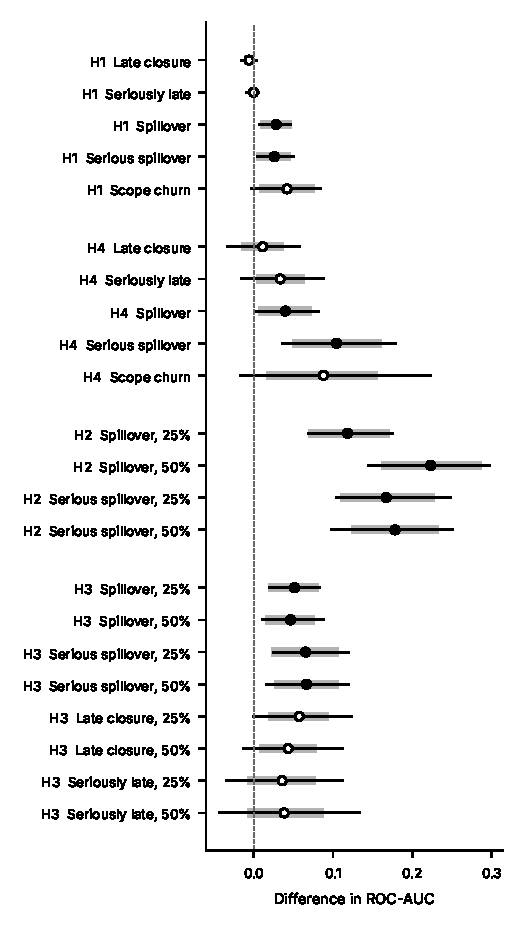
\includegraphics[width=\columnwidth]{fig_primary.pdf}
\caption{The hypothesis comparisons of Table~\ref{tab:hyp} on the full cohort. Dot: difference in AUC (filled where the project-level interval is above zero). Black line: 95\% interval over projects. Grey bar: 95\% interval over sprints.}
\label{fig:primary}
\end{figure}

\emph{H1, new features: holds for spillover only, and does not replicate.} The new features add \dPTNewSp{} \cPTNewSp{} for spillover, which survives the Holm adjustment, but only \dPCNewSp{} \cPCNewSp{} on the confirmation set. For serious spillover the gain is \dPTNewSs{} \cPTNewSs, with the same sign in all three models. For the two late labels it is about zero, as predicted (for seriously late the interval ends just below zero). Within projects the spillover gain is the same size (Section~\ref{sec:within}). We read H1 as a small gain for spillover that we cannot confirm.

\emph{H2, burndown shape: holds everywhere.} Ours beats worki by 0.13 to 0.19 AUC on both spillover labels at both checkpoints, in the full cohort and on the confirmation set. Because the two sets were built for different tasks (Section~\ref{sec:protocol}), the size of this gap says little by itself; the fair test is in Section~\ref{sec:fair}.

\emph{H3, planning context: right direction, too weak to hold.} Ours beats choet for every outcome, by 0.03 to 0.09, so in \NHThreeOver{} of the \NHThree{} comparisons the gain is above the 0.05 ceiling we predicted. On the full cohort the project-level interval clears zero clearly only for seriously late at 50\%; for the spillover labels it sits on zero. On the confirmation set the gain is larger and holds for both spillover labels. Section~\ref{sec:fair} shows where it comes from.

\emph{H4, new labels: fails where it was most specific.} We predicted that history would add nothing to serious spillover beyond scope. It adds \dPTHistSs{} \cPTHistSs{} on the time split, \dPLHistSs{} \cPLHistSs{} under leave-one-project-out testing and \dPCHistSs{} on the confirmation set. It does not survive the Holm adjustment, but it holds under leave-one-project-out testing and every robustness variant, and replicates on the confirmation set. All of these scores are pooled over projects, though, and within projects the gain falls to \dPWHistSs{} \cPWHistSs{} (Section~\ref{sec:within}). History tells which teams leave more work over, not which of a team's sprints will. Seriously late and scope churn do not hold.

\subsection{Planning time}

Table~\ref{tab:planauc} gives the AUC of the planning-time sets. Late closure is hard: scope alone reaches \aPTLcScope, and the best set \aPTLcNew. The binomial model of Section~\ref{sec:theory} predicts that history should beat scope by more for serious spillover than for plain spillover. It does: strict minus scope is \dPTStrSp{} for spillover against \dPTStrSs{} for serious spillover on the time split, and \dPLStrSp{} against \dPLStrSs{} under leave-one-project-out testing. Plain spillover is mostly a matter of how many issues were committed; serious spillover is mostly a matter of which team committed them. The same model also limits what history can do, which we saw only after the full run. If $q_s$ is a property of the team and changes slowly, history separates teams but not the sprints of one team. Section~\ref{sec:within} checks this. The median-based serious-spillover label shows the same pattern more clearly: strict+new scores \aPTSmNew{} against \aPTSmScope{} for scope.

\begin{table}[t]
\centering
\small
\caption{Planning-time ROC-AUC, gradient boosting. Time: per-project time split. LOPO: leave one project out (no project feature).}
\label{tab:planauc}
\setlength{\tabcolsep}{4pt}
\begin{tabular}{@{}lrrrrrr@{}}
\toprule
& \multicolumn{3}{c}{Time split} & \multicolumn{3}{c}{LOPO} \\
\cmidrule(lr){2-4}\cmidrule(l){5-7}
Outcome & scope & strict & +new & scope & strict & +new \\
\midrule
\tabinput{tables/planning_auc.tex}
\bottomrule
\end{tabular}
\end{table}

AUC is high for spillover partly because the label is \PosSp\% positive. Only \NegSp{} nonempty test sprints finish everything they committed (\NegSs{} for serious spillover). Average precision for finding those sprints (Table~\ref{tab:apneg} in the Appendix) is several times the base rate but well below one, so the spillover models are much better at confirming the common outcome than at spotting the rare good sprint.

\subsection{During the sprint}
\label{sec:fair}

Table~\ref{tab:inauc} gives the in-sprint AUC, on the nonempty sprints still open at the checkpoint (\InTestA{} test sprints at 25\%, \InTestB{} at 50\%). Table~\ref{tab:fair} gives the fair comparisons.

\begin{table}[t]
\centering
\small
\caption{In-sprint ROC-AUC at 25\% and 50\% of the planned duration, gradient boosting, time split.}
\label{tab:inauc}
\footnotesize
\setlength{\tabcolsep}{2.4pt}
\begin{tabular}{@{}llrrrrrr@{}}
\toprule
Outcome & At & scope & worki & choet & +ctx & ours & +worki \\
\midrule
\tabinput{tables/insprint_auc.tex}
\bottomrule
\end{tabular}
\end{table}

\begin{table*}[t]
\centering
\footnotesize
\caption{What each family adds to the others during the sprint: differences in AUC with 95\% intervals over projects (gradient boosting, time split).}
\label{tab:fair}
\setlength{\tabcolsep}{4pt}
\begin{tabular}{@{}llccc@{}}
\toprule
Outcome & At & Burndown shape added & Planning context added & Our progress counts \\
& & ours+worki $-$ ours & choet+ctx $-$ choet & ours $-$ choet+ctx \\
\midrule
\tabinput{tables/fair.tex}
\bottomrule
\end{tabular}
\end{table*}

\emph{Burndown shape adds nothing.} Adding the worki set to ours changes AUC by at most \AddMax{} for any outcome at either checkpoint. On its own the worki set ranks worse than committed scope, with intervals below zero, for late closure at 25\% (\dITWsLcA{} \cITWsLcA), for seriously late at both checkpoints and for spillover at 50\%.

\emph{Planning context adds little once progress counts are in.} Added to the choet counts, planning context changes AUC by \dITCtxSpA{} and \dITCtxSpB{} for spillover and \dITCtxSsA{} and \dITCtxSsB{} for serious spillover; none of these intervals clears zero. Under leave-one-project-out testing it helps serious spillover (\dILCtxSsA{} \cILCtxSsA{} at 25\%). For seriously late at 50\% it adds \dITCtxSlB{} \cITCtxSlB.

\emph{Our progress counts add a little beyond theirs for serious spillover} at 50\% (\dITProgSsB{} \cITProgSsB), and on the confirmation set at both checkpoints. The H3 gap is therefore partly progress counts and partly context, and neither part is large.

\emph{The spillover labels are where the signal is.} Serious spillover goes from \aPTSsNew{} at planning time to \aITSsAOurs{} at 25\% and \aITSsBOurs{} at 50\%. For late closure our set reaches only \aITLcAOurs{} and \aITLcBOurs, against \aITLcAScope{} and \aITLcBScope{} for scope alone on the same sprints.

\subsection{A model with no learning}

Table~\ref{tab:binomial} scores the binomial model of Section~\ref{sec:theory} as a predictor. For each sprint, $q_s$ is the pooled completion rate of the team's last three finished sprints known at the start, or the training-set rate where there is no history. Nothing else is fitted. Its AUC is \aBinSp{} against \aBinGbSp{} for gradient boosting on spillover (difference \dGbBinSp{} \cGbBinSp) and \aBinSs{} against \aBinGbSs{} on serious spillover (\dGbBinSs{} \cGbBinSs). The two cannot be told apart. For serious spillover the binomial model beats scope alone by \dBinScopeSs{} \cBinScopeSs. On the confirmation set the gap to gradient boosting is wider (\dGbBinCSp{} and \dGbBinCSs, intervals \cGbBinCSp{} and \cGbBinCSs) and the binomial model still beats scope for serious spillover (\dBinScopeCSs{} \cBinScopeCSs). Most of what the learned model adds over scope at planning time is therefore an estimate of one number per team.

\begin{table}[t]
\centering
\small
\caption{The binomial model as a predictor on the nonempty test sprints. AUC and calibration slope (1 is ideal).}
\label{tab:binomial}
\setlength{\tabcolsep}{3pt}
\begin{tabular}{@{}lrrrr@{}}
\toprule
& \multicolumn{2}{c}{Spillover} & \multicolumn{2}{c}{Serious sp.} \\
\cmidrule(lr){2-3}\cmidrule(l){4-5}
Model & AUC & Slope & AUC & Slope \\
\midrule
\tabinput{tables/binomial.tex}
\bottomrule
\end{tabular}
\end{table}

Its probabilities are another matter. The calibration slopes are \sBinSp{} and \sBinSs, so the binomial model is far too sure of itself. Table~\ref{tab:variance} in the Appendix shows why. In every band of sprint size the observed variance of the carry ratio exceeds the binomial variance, by a factor of \VarRatioSmall{} for sprints of one to three issues and \VarRatioLarge{} for sprints of 16 or more. A gap that grows with sprint size is what Proposition~\ref{prop:overdisp} predicts when $r > 0$. The ratio of observed to binomial variance over the training sprints, the quantity behind Tarone's test of binomial fit \cite{tarone1979}, is \DispRatio, and the maximum-likelihood estimate is $r = \Rhat$ (likelihood-ratio statistic \LRstat{} against $r = 0$). The beta-binomial model matches the observed variance for large sprints (\VarBetaLarge{} against \VarObsLarge) and raises the slopes to \sBetaSp{} and \sBetaSs, at a small cost in ranking (\mBetaCostSp{} and \mBetaCostSs{} AUC). Neither is as well calibrated as gradient boosting (slopes \sGbSp{} and \sGbSs). The learned model earns its keep through its probabilities far more than through its ranking.

\subsection{Within projects}
\label{sec:within}

Every AUC so far is pooled over the test sprints of all \NProj{} projects. A pair of sprints from two different projects counts as much as a pair from the same project, so a model can score well just by knowing which projects leave more work over. That is useful to someone who watches many teams. A team that uses a warning tool sees only its own sprints. Table~\ref{tab:within} therefore repeats the main comparisons on the same models and test sprints, counting only pairs of sprints from the same project, with the same project-level bootstrap. We added this analysis after the full run.

\begin{table*}[t]
\centering
\footnotesize
\caption{Pooled and within-project differences in AUC with 95\% intervals over projects (gradient boosting, time split). Pooled: all test sprints, as in the rest of the paper. Within: only pairs of sprints from the same project. $k$: projects with both classes in the test set. Planning time unless a checkpoint is given.}
\label{tab:within}
\setlength{\tabcolsep}{5pt}
\begin{tabular}{@{}llccr@{}}
\toprule
Comparison & Outcome & Pooled & Within & $k$ \\
\midrule
\tabinput{tables/within.tex}
\bottomrule
\end{tabular}
\end{table*}

The in-sprint findings hold. Progress counts beat burndown shape by \dIWWkSpB{} \cIWWkSpB{} for spillover at 50\%, and burndown shape still adds nothing. The new features keep their gain for spillover (\dPWNewSp{} \cPWNewSp). The history gain does not. For serious spillover it falls from \dPTHistSs{} to \dPWHistSs{} \cPWHistSs, and for late closure the history-aware set ranks a team's own sprints worse than scope alone (\dPWHistLc{} \cPWHistLc). This is the binomial reading again. The last three sprints estimate a team's completion rate, which separates teams well, but a rate that changes slowly says little about which of the team's next sprints will go badly. It also bears on the outside test of Section~\ref{sec:external}, which averages AUC within each outside project. Within TAWOS projects the history-aware set ranks serious spillover at \wPTSsNew{} against \wPTSsScope{} for scope, so the outside test asked history for a gain it does not show at home either.

\subsection{What a warning is worth}

A difference of 0.03 AUC means little to a team. Table~\ref{tab:budgets} in the Appendix asks a concrete question instead: if someone can look into only 10\% or 20\% of the sprints, how many of the ones flagged are real problems? The budgets are set over all test sprints, so this is the view of someone who oversees many teams, not of one team. For serious spillover in its median form, the history-aware model raises the hit rate among the top 10\% from \bSmTenScope\% to \bSmTenNew\% (\bSmTenExtra{} more real problems among \bSmTenFlag{} flagged sprints), against a base rate of \bSmTenBase\%. For late closure the gain is \bLcTenScope\% to \bLcTenNew\%.

Table~\ref{tab:nb} applies the net benefit (\ref{eq:nb}) on the \NbN{} sprints scored at all three stages. Never warning scores zero. For serious spillover, warning on every sprint is almost as good as any model unless warnings are costly: at $p^{*} = 0.5$ warning on all sprints gives \nbSsHalfAll{} against \nbSsHalfPlan{} at planning and \nbSsHalfB{} at 50\%. Only at $p^{*} = 0.9$, where a warning must be nearly certain to pay, does the model clearly add value (\nbSsNinePlan{} at planning and \nbSsNineB{} at 50\%, against \nbSsNineAll{} for warning on all). There, waiting until 50\% of the sprint pays only if a warning at that point still averts at least \beSsNineB{} of what an early warning would. For late closure the picture is reversed: warning on all sprints loses at any threshold above the base rate, the planning-time model gains a little (\nbLcThreePlan{} at $p^{*} = 0.3$, \nbLcHalfPlan{} at 0.5), and the in-sprint models gain no more than the planning model, so waiting never pays. Fig.~\ref{fig:reliability} shows the calibration behind these numbers.

\begin{table}[t]
\centering
\small
\caption{Net benefit (\ref{eq:nb}) per sprint, in units of the averted failure cost, on the same \NbN{} test sprints. All: warn on every sprint. Never warning scores 0.}
\label{tab:nb}
\setlength{\tabcolsep}{3pt}
\begin{tabular}{@{}lrrrrr@{}}
\toprule
Outcome & $p^{*}$ & All & Planning & 25\% & 50\% \\
\midrule
\tabinput{tables/net_benefit.tex}
\bottomrule
\end{tabular}
\end{table}

\begin{figure}[!htb]
\centering
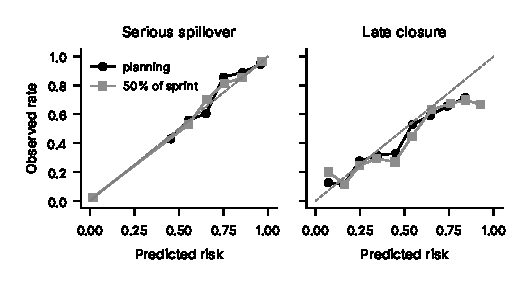
\includegraphics[width=\columnwidth]{fig_reliability.pdf}
\caption{Reliability of the gradient-boosting risk on the sprints of Table~\ref{tab:nb}: mean predicted risk against the observed rate, in bins of width 0.1 with at least ten sprints.}
\label{fig:reliability}
\end{figure}

\subsection{Outside projects}
\label{sec:external}

Table~\ref{tab:external} trains on all of TAWOS and tests on each outside project with at least five sprints in each class. We find no evidence of transfer. For the two spillover labels, where history helped most inside TAWOS, scope alone scores \eSpScope{} and \eSsScope, and the history-aware sets score lower. For late closure all three sets sit between \eLcStrict{} and \eLcScope. Only \eKSp{} outside projects are testable for spillover, and the spread across projects is large, so we can only say that we see no transfer, not that there is none. We cannot tell whether the cause is the new organisations, because two simpler reasons could explain it. The outside test scores ranking within each project, where history adds little even inside TAWOS (Section~\ref{sec:within}), and its feature sets leave out story points, which MariaDB does not record.

\begin{table}[t]
\centering
\footnotesize
\caption{Outside projects: mean $\pm$ s.d.\ of per-project AUC, gradient boosting trained on all TAWOS sprints. $k$: projects with at least five sprints in each class.}
\label{tab:external}
\setlength{\tabcolsep}{3pt}
\begin{tabular}{@{}lrccc@{}}
\toprule
Outcome & $k$ & scope & strict & strict+new \\
\midrule
\tabinput{tables/external.tex}
\bottomrule
\end{tabular}
\end{table}

\subsection{Robustness}
\label{sec:robust}

Table~\ref{tab:robust} in the Appendix repeats the main planning-time comparisons under five variants. \emph{Tuning:} with a small grid chosen on a time-ordered validation slice, the new features add \dPUNewSp{} \cPUNewSp{} for spillover and history beats scope for serious spillover by \dPUHistSs{} \cPUHistSs. \emph{A single calendar cut} in early 2018 (train on sprints whose outcome was known before it, test on sprints that start after it, \CutProj{} projects): \dPKNewSp{} \cPKNewSp{} and \dPKHistSs{} \cPKHistSs. \emph{Without \RestrictedProj}, the two projects whose sprints mostly finish nothing although they pass the measurability check: \dPRNewSp{} \cPRNewSp{} and \dPRHistSs{} \cPRHistSs. \emph{Before the measurability check}, on all \NProjExport{} projects, the new features added more for serious spillover and less for spillover, which is why we report the check as a contribution. \emph{Sprint-history coverage:} on the \HistProj{} projects where at least 85\% of issues ever placed in a sprint have a sprint history, the new features add \dPHNewSp{} \cPHNewSp{} for spillover and history beats scope for serious spillover by \dPHHistSs{} \cPHHistSs. Burndown shape added to ours changes AUC by at most \HistAddMax, and planning context added to the choet counts gains more than on the full cohort (\dIHCtxSpA{} \cIHCtxSpA{} for spillover at 25\%), so the weak planning-context result may partly reflect missing sprint history rather than a weak signal. \emph{Story-point provenance:} on test sprints with no story-point fallback, the new features add \dPFNewSp{} \cPFNewSp{} for spillover and history beats scope for serious spillover by \dPFHistSs{} \cPFHistSs. The five time-ordered repeats agree with the time split (strict+new scores \repSp{} for spillover, \repSs{} for serious spillover and \repLc{} for late closure). Calibration is in Table~\ref{tab:calibration}: slopes from \SlopeSpMin{} to \SlopeSpMax{} for the spillover labels and from \SlopeLateMin{} to \SlopeLateMax{} for the late labels, which are overconfident.

\section{Discussion}
\label{sec:discussion}

\subsection{What a team can take from this}

During a sprint, simple progress counts (how much is done, how much is left, how fast it is going) carry nearly all of the signal, within a team as well as across teams, and their warnings for leftover work are close to calibrated. Burndown-shape indicators add nothing on top of them.

Before a sprint starts, the picture depends on who is looking. Someone who oversees many teams learns most from each team's recent completion rate, and the binomial model gives that ranking with nothing learned, though its probabilities need the beta-binomial correction or a learned model before anyone acts on them. A single team learns little from its own history that the size of the sprint does not already say. The new features help a little with plain spillover, but that gain did not hold on the confirmation set.

We see no sign that a model trained on other organisations' teams does better than a size rule, and a threshold carried from one team to another changes what a miss is worth (Proposition~\ref{prop:youden}). For outcomes as common as spillover, the decision analysis adds a further caution: unless a warning is costly, warning on every sprint is nearly as good as any model.

\subsection{Why lateness is hard}

Late closure is the moment someone pressed ``Complete sprint'' in Jira. That depends on meetings, holidays and habit as much as on the work, and no feature family we tried moves it much. We keep it for continuity, but we would not build a tool on it. Seriously late is no easier to rank, and its scores are among the worst calibrated in the study.

\subsection{Threats to validity}
\label{sec:threats}

\emph{Construct.} The labels come from Jira fields, not from asking teams whether a sprint went badly. Late closure and seriously late measure when a sprint was closed in the tool. Spillover counts issues, not effort. The median nonempty sprint leaves \CarryMedPct\% of its committed issues unresolved at the planned end, and \CleanNothingPct\% of nonempty sprints resolve none. In open-source projects an issue is often resolved at a release or a merge rather than when the work stops, so the carry ratio partly measures when a project resolves issues, not only how much work was left. The measurability check catches only issues closed with no date at all; a project that sets resolution dates late passes it and still overstates spillover. We think this is the largest threat to the spillover labels, and only the teams themselves can settle it.

\emph{Internal.} The reconstruction depends on the change log. Where it is missing, story points fall back on the exported value; we measured the share and repeated the main comparisons without it. Issue type, priority and assignee are left out because only their final values exist, which also means the choet set lacks team and issue features its authors used. The strict, choet+ctx and ours sets carry the project as a feature; leave-one-project-out testing removes it.

\emph{Hypotheses and analysis choices.} The hypotheses were written after a development run on eight projects. Several choices were made after the full run: the measurability check, the choet+ctx set, the Holm adjustment, the confirmation set, the tuned and calendar-cut variants, the within-project analysis and the decision analysis. All are logged with dates and reasons, and we report their effect whichever way it went. The confirmation set is our main answer to this threat: the in-sprint and serious-spillover results hold there, the new-features result does not. It is not an independent replication, though. Its \ConfProj{} projects are part of the full cohort, so the two estimates share \ConfSprints{} sprints, and every choice made after the full run was made with those projects in view.

\emph{Conclusion.} The project-level interval resamples only \NProj{} clusters, so it is wide. We treat a result as holding only when the project interval clears zero, and report the adjusted values beside it.

\emph{External.} All projects are open source, and a handful of organisations contribute most TAWOS projects. The outside test covers two more organisations and ten projects, few of which have enough sprints in both classes for every label.

\section{Conclusion}

Under one leakage-aware protocol, and after checking that the outcomes can be measured, the kinds of signal used in the sprint-risk literature differ sharply. Progress counts dominate during a sprint and burndown shape adds nothing. Team history tells teams apart, but adds little to ranking one team's own sprints and nothing for when a sprint is closed, and we see no sign that it helps on another organisation's projects. Because every AUC in this literature is pooled over projects, results like ours should be reported within projects too. The formal setting gives simple reasons for these patterns: empty sprints inflate AUC by an exact amount, a fitted threshold carries a hidden cost ratio, the choice between ``any'' and ``serious'' spillover decides whether history can matter, a completion rate that belongs to the team says little about which of that team's sprints will go badly, and issues that do not finish independently explain why a model with no learning ranks well but cannot give trustworthy probabilities. The obvious next step is to ask teams whether the sprints these models flag are the ones they would have wanted to hear about.

\section*{Data Availability}

Code, export queries, the measurability and reconstruction checks, the reconstructed frames, every result file and the dated study plan with its change log are at \url{https://github.com/hani-ziad/journal-ieee-access-2027}. TAWOS \cite{tawos} is released under the Apache License 2.0 for research use. The repository includes the eight-project extract used for development and the SQL that makes the full extract from the public TAWOS database; the full extract is too large for the repository and is available from the author. The outside projects' issues come from the public Jira sites of MariaDB and MongoDB; we do not redistribute them, but the repository includes the scripts that pull and convert them.

\appendix

\section*{Appendix: Further Results}

\begin{table}[h]
\centering
\small
\caption{Variance of the carry ratio around $1 - \hat q_s$ on the training sprints, by committed issues: observed, binomial (\ref{eq:ratio}) and beta-binomial (\ref{eq:overdisp}) with $r = \Rhat$.}
\label{tab:variance}
\begin{tabular}{@{}lrrrr@{}}
\toprule
Issues & Sprints & Observed & Binomial & Beta-bin. \\
\midrule
\tabinput{tables/binomial_variance.tex}
\bottomrule
\end{tabular}
\end{table}

\begin{table}[h]
\centering
\small
\caption{Warning budgets at planning time: share of flagged sprints that are real problems (\%) when the top 10\% or 20\% of test sprints by risk are flagged. Base: positive rate.}
\label{tab:budgets}
\setlength{\tabcolsep}{3pt}
\begin{tabular}{@{}lrrrrr@{}}
\toprule
Outcome & Flag & Base & scope & strict & +new \\
\midrule
\tabinput{tables/budgets.tex}
\bottomrule
\end{tabular}
\end{table}

\begin{table}[h]
\centering
\small
\caption{Average precision for finding the sprints that do \emph{not} spill (planning time, gradient boosting, time split). Base: share of such sprints among the nonempty test sprints.}
\label{tab:apneg}
\setlength{\tabcolsep}{3pt}
\begin{tabular}{@{}lrrrrr@{}}
\toprule
Outcome & $n$ & Base & scope & strict & +new \\
\midrule
\tabinput{tables/apneg.tex}
\bottomrule
\end{tabular}
\end{table}

\begin{table}[h]
\centering
\footnotesize
\caption{Main planning-time differences in AUC under each robustness variant. Columns: new features (strict+new $-$ strict) and history over scope (strict+new $-$ scope) for spillover (Sp), serious spillover (Ss) and late closure (Lc). $^{*}$: project-level interval above zero.}
\label{tab:robust}
\scriptsize
\setlength{\tabcolsep}{2pt}
\begin{tabular}{@{}lrrrrrr@{}}
\toprule
& \multicolumn{3}{c}{New features} & \multicolumn{3}{c}{History over scope} \\
\cmidrule(lr){2-4}\cmidrule(l){5-7}
Variant & Sp & Ss & Lc & Sp & Ss & Lc \\
\midrule
\tabinput{tables/robust.tex}
\bottomrule
\end{tabular}
\end{table}

\begin{table}[h]
\centering
\small
\caption{Calibration on the time-split test set, gradient boosting. Ref.: Brier score of the test prevalence. ECE: expected calibration error, ten bins.}
\label{tab:calibration}
\setlength{\tabcolsep}{3.5pt}
\begin{tabular}{@{}llrrrr@{}}
\toprule
Outcome & Stage & Brier & Ref. & ECE & Slope \\
\midrule
\tabinput{tables/calibration.tex}
\bottomrule
\end{tabular}
\end{table}
